

The overall data flow of the \instname\ pipeline is displayed in Figure \ref{fig:reduction_cascade}.

 
\begin{figure}[h!]
\centering
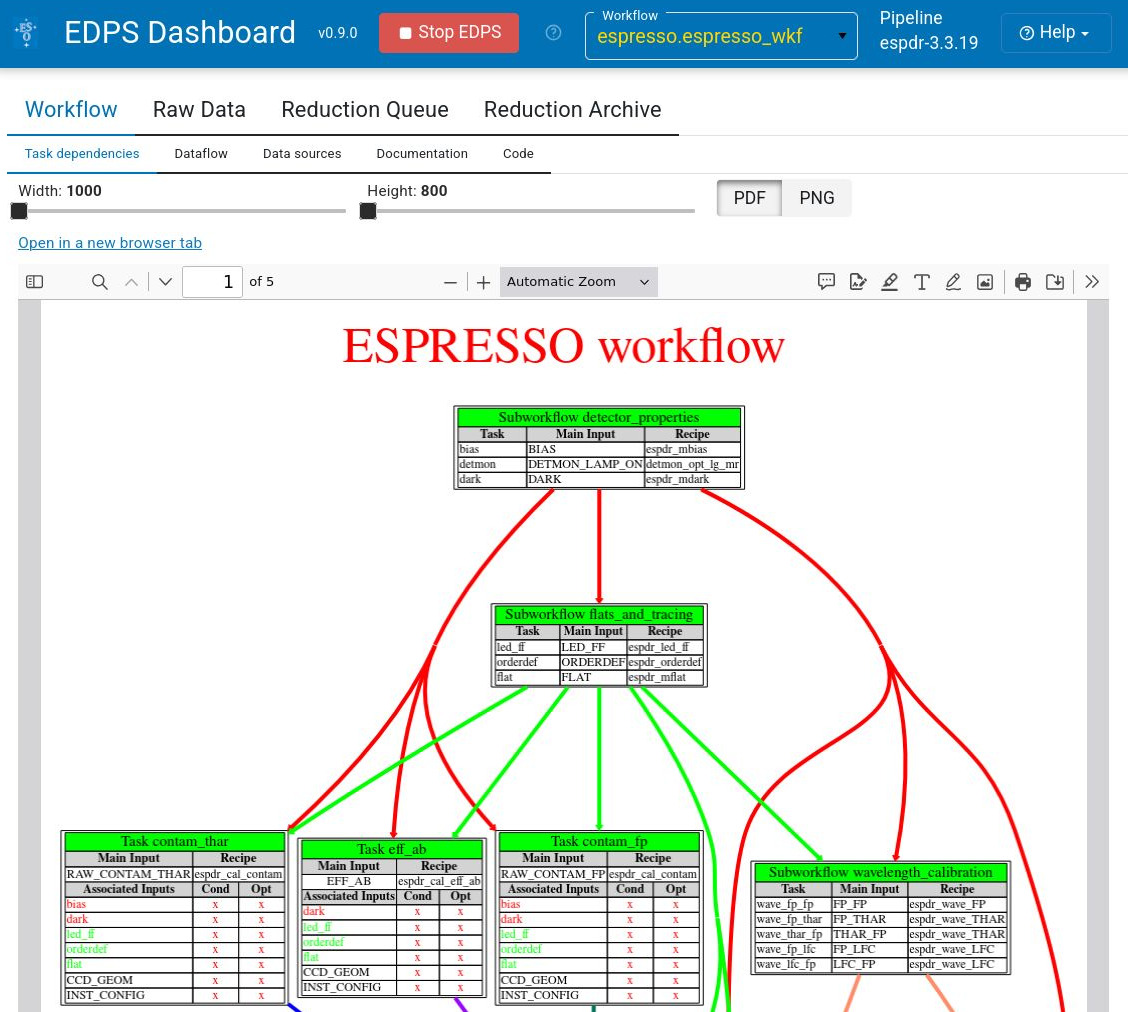
\includegraphics[width=0.9\textwidth]{../instrument_tutorial/figures/reduction_cascade.jpg}
\caption{The data reduction cascade of the \instname\ workflow.}
\label{fig:reduction_cascade}
\end{figure}



The reduction cascade is organized in tasks, which represent
well-defined steps in the process. Tasks can be grouped inside
sub-workflows.  Each task runs a recipe; the detailed description of
the algorithms, input, outputs and recipe parameters used in each
recipe are available in the pipeline manual. Here, we present only the
description of most important features.

The \wkfname\  \edps\ workflow is designed to execute the tasks that
deliver the final reduced data cube for each dataset. It can be either
the product of a single exposure, or the combination of multiple
exposures. Only calibrations needed by the selected the scientific
exposures are processed.

It is possible to set \edps\ to perform the data reduction until a
certain step of the reduction chain (e.g. to reduce only standar
stars, or only flat fields).  This is done by specifying the desired
tasks in the field {\bf Select reduction target} of the {\bf Raw Data}
tab.

The reduction steps of the \wkfname\ workflow are listed below. Before
starting the reduction, the parameters of the recipes associated to
each task can be configured by pressing the button

\includegraphics[width=0.8cm]{../common/figures/configure_dataset.jpg}
close to each dataset configuration.
See for more info on the configuration editor \ref{sec:configuration_editor}

